\documentclass{article}
\usepackage{stmaryrd}
\usepackage{graphicx}
\usepackage{float}

\title{Report, Kinetic project}
\author{Dorian Geraldes Pereira, Axel Demuth}
\date{March 2024}

\begin{document}
\maketitle
\tableofcontents
\newpage


\section{Objectives}
To be able to solve equations on a mesh, we need it to be watertight.

The objectives of the project are:

\begin{itemize}
    \item Repair mesh to make them watertight
   

    \begin{itemize}
        \item watertight building model
        

        \item watertight urban model
    \end{itemize} 
\end{itemize} 

In our project we will have to use files in IFC format containing building meshes that are not watertight in an algorithm repairing
geometric error in a kinetic data structures. We will have to find a way to keep the label 
on the surfaces in the algorithm or relabel every surfaces at the end.
we can see here an example of what we will need to do:

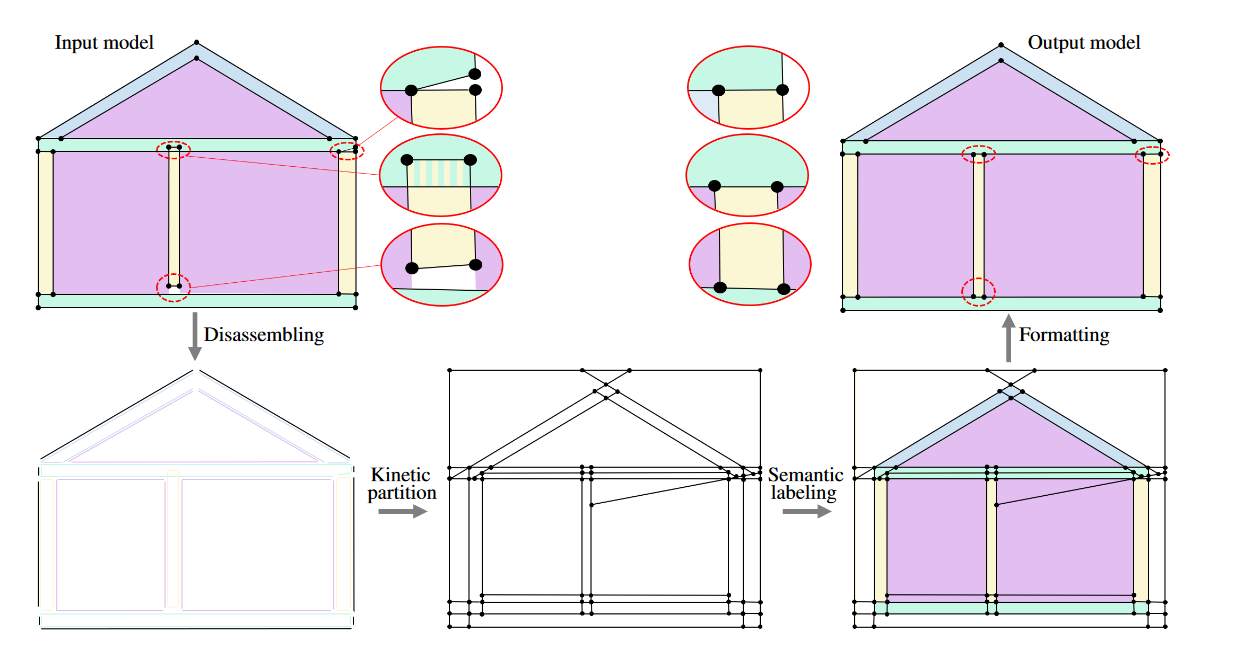
\includegraphics[scale = 0.37]{../images/example_algorithm_2.png}



\section{Tools}
\subsection{CGAL}
CGAL is a comprehensive package for geometry algorithms, providing various data structures and algorithms for working on polygons, surfaces, mesh generation, and more.
It offers a wide range of functionalities for geometric processing and analysis in various fields such as computer graphics, computational geometry, and geometric modeling.


\subsection{Kinetic}

Kinetic algorithms is a package from CGAL that allows working on meshes with some holes in them. When applied to the mesh, the Kinetic algorithms will 'extend' some surfaces to fill the mesh and make it watertight. 
Here's what the algorithm is capable of:

\begin{figure}[h]
    
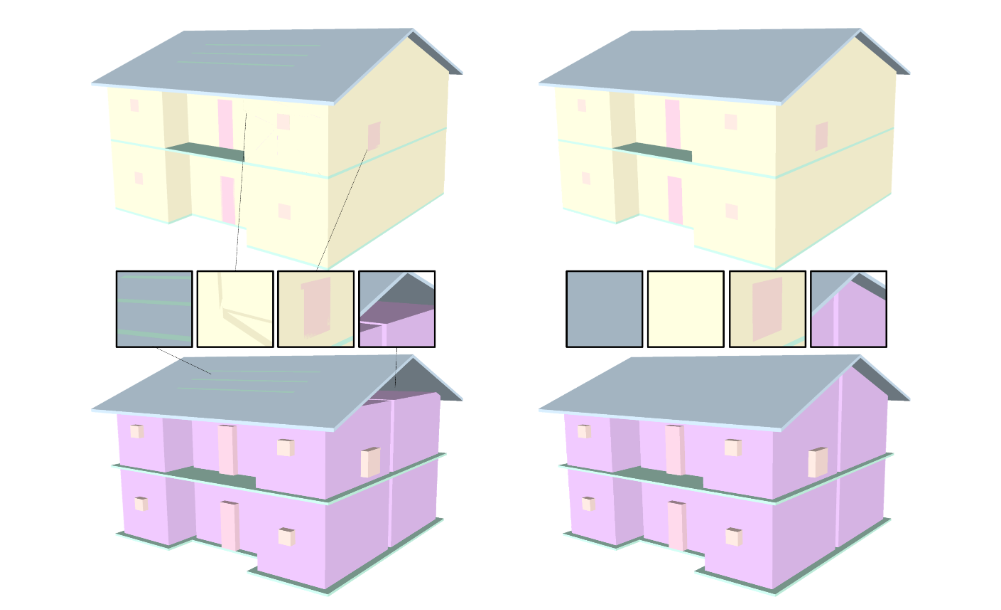
\includegraphics[scale =   0.3 ]{../images/example_algorithm.png}



\end{figure}

To utilize the algorithm, we employ one from CGAL. Given a set of parameters and a file containing a point cloud along with the associated normals to the points,
the algorithm is applied. We were fortunate to have a meeting with Florent Lafarge, one of the creators of the algorithm,
who explained to us which parameters are crucial for analysis and how each one can significantly influence the results.
Two parameters stand out as particularly important: 'dist' and 'pmin.' 'Pmin' represents the number of points used to construct a plane, 
while 'dist' indicates the distance between two points required to consider them for plane construction.

In order to understand how these parameters affect the outcome, we will examine the same point cloud while varying the value of 'pmin' first and then varying 'dist.'
The algorithm produces .off files as output, which can be visualized using software such as MeshLab.

\newpage
The original point cloud represents this building:
\vspace{\baselineskip}

\begin{center}
    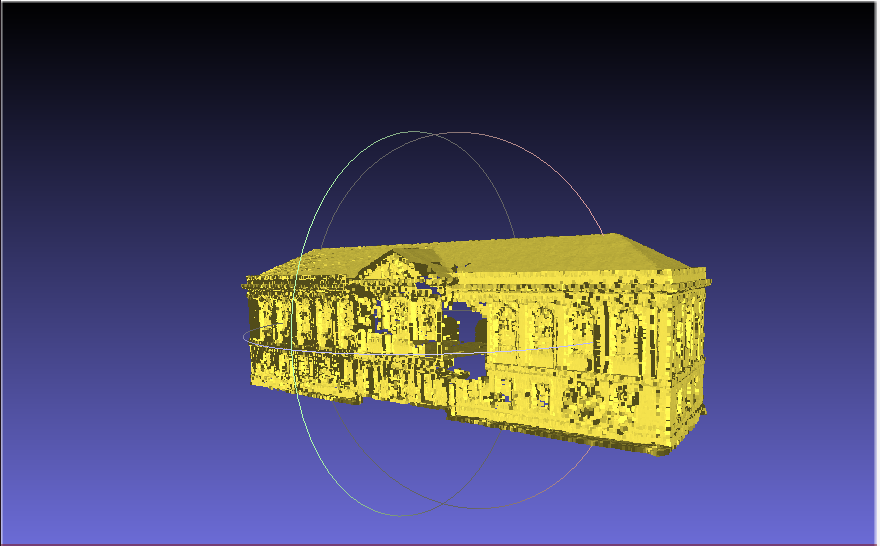
\includegraphics[scale=0.20]{../images/screen_kinetic/building.png} 
\end{center}



\begin{figure}[H]
    \centering
    \begin{minipage}[b]{0.45\textwidth}
      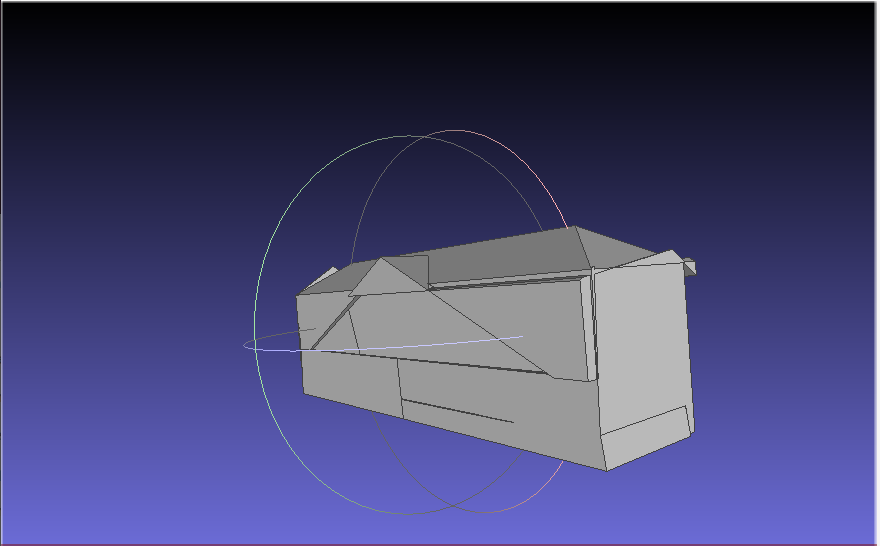
\includegraphics[width=\textwidth]{../images/screen_kinetic/dist1_pmin220.png}
      \caption{dist1\_pmin220}
      \label{fig:dist1_pmin220}
    \end{minipage}
    \hfill
    \begin{minipage}[b]{0.45\textwidth}
      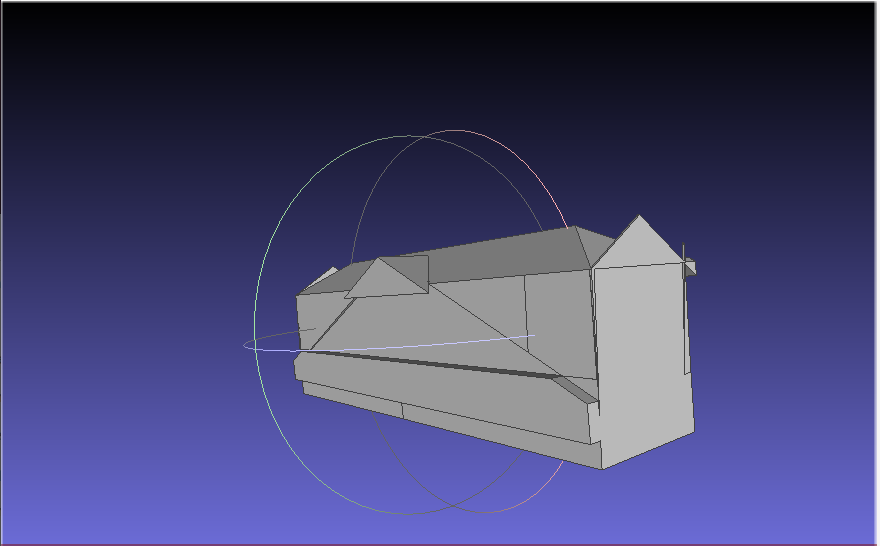
\includegraphics[width=\textwidth]{../images/screen_kinetic/dist1_pmin250.png}
      \caption{dist1\_pmin250}
      \label{fig:dist1_pmin250}
    \end{minipage}
    \hfill
    \begin{minipage}[b]{0.45\textwidth}
      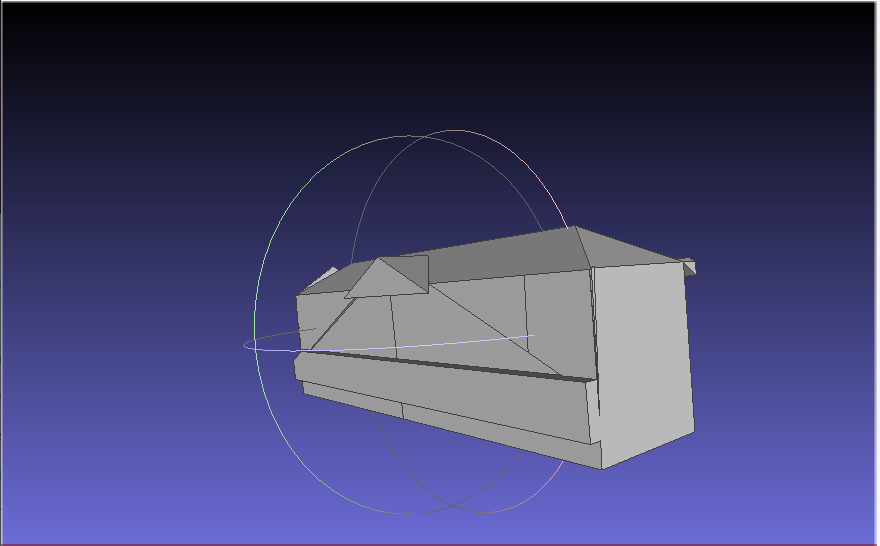
\includegraphics[width=\textwidth]{../images/screen_kinetic/dist1_pmin280.png}
      \caption{dist1\_pmin280}
      \label{fig:dist1_pmin280}
    \end{minipage}
    \hfill
    \begin{minipage}[b]{0.45\textwidth}

        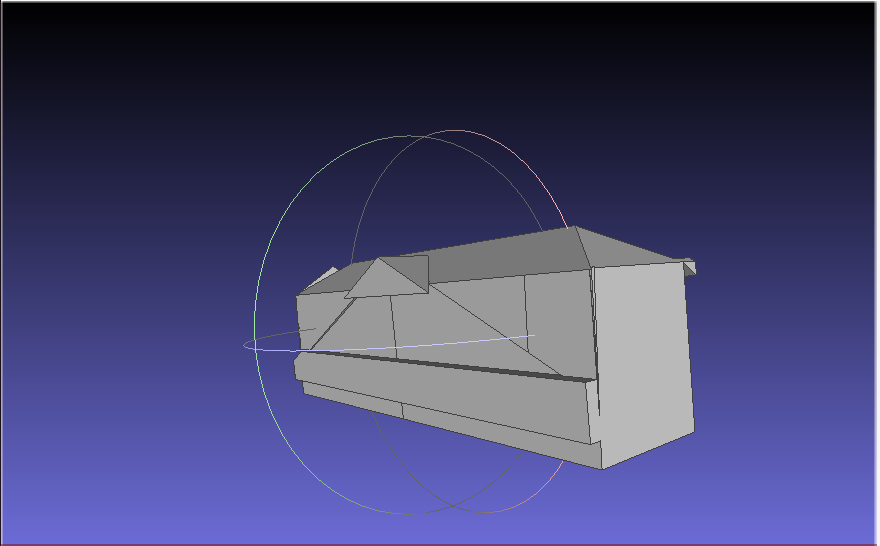
\includegraphics[width=\textwidth]{../images/screen_kinetic/dist1_pmin300.png}
        \caption{dist1\_pmin300}
        \label{fig:dist1_pmin300}
      \end{minipage}
  \end{figure}
  
  First, it's important to understand that setting 'pmin' too low can lead to errors. Subsequently,if 'pmin' is too small, we may not capture enough structural detail,
  whereas setting 'pmin' too high may cause planes to overlap, resulting in loss of information



  \begin{figure}[H]
    \centering
    \begin{minipage}[b]{0.45\textwidth}
      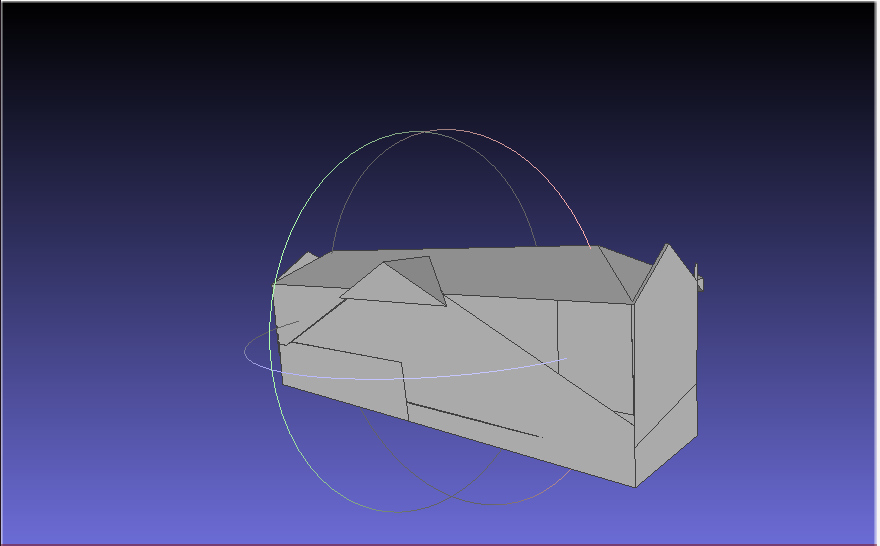
\includegraphics[width=\textwidth]{../images/screen_kinetic/dist1_5_pmin_250.png}
      \caption{dist15\_pmin250.png}
      \label{fig:dist15_pmin220}
    \end{minipage}
    \hfill
    \begin{minipage}[b]{0.45\textwidth}
      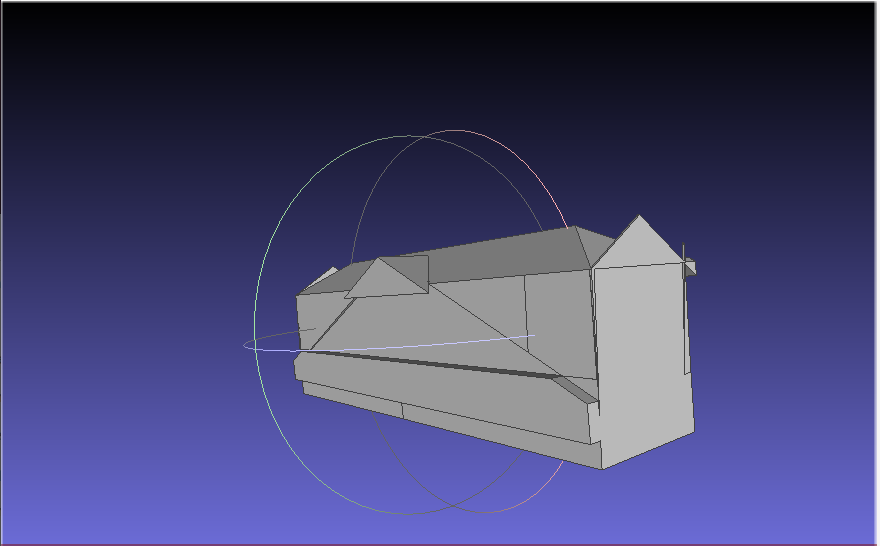
\includegraphics[width=\textwidth]{../images/screen_kinetic/dist1_pmin250.png}
      \caption{dist1\_pmin250}
      \label{fig:dist1_pmin250}
    \end{minipage}
    \hfill
    \begin{minipage}[b]{0.45\textwidth}
      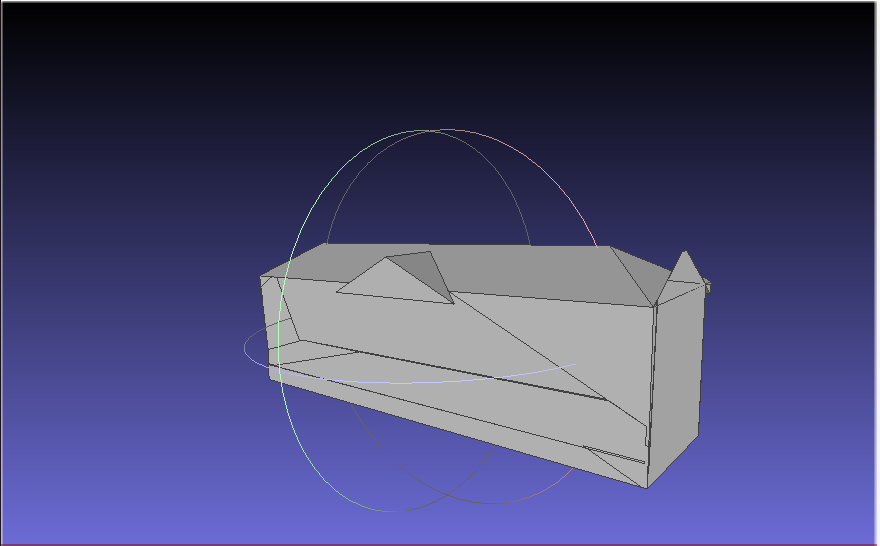
\includegraphics[width=\textwidth]{../images/screen_kinetic/dist_0_3_pmin_250.png}
      \caption{dist03\_pmin250}
      \label{fig:dist03_pmin250}
    \end{minipage}
    \hfill
    \begin{minipage}[b]{0.45\textwidth}

        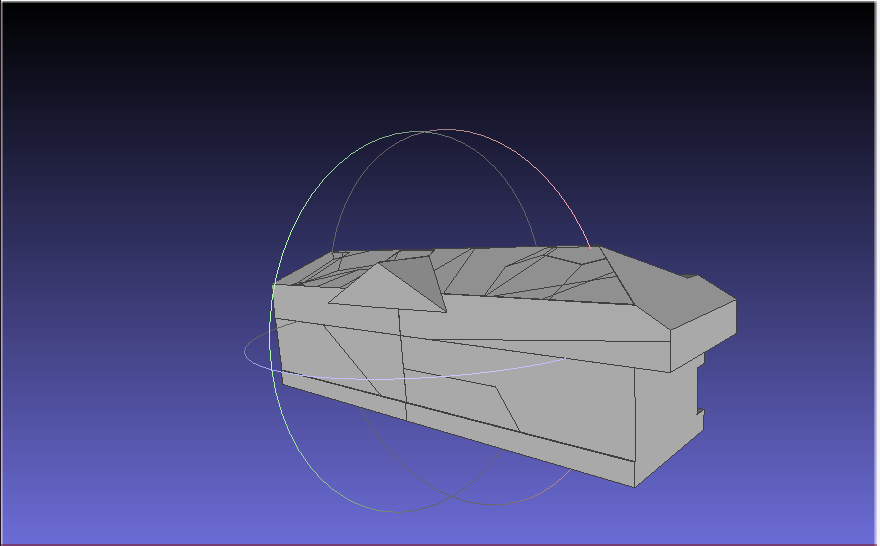
\includegraphics[width=\textwidth]{../images/screen_kinetic/dist_001_pmin_250.png}
        \caption{dist001\_pmin250}
        \label{fig:dist1_pmin300}
      \end{minipage}
    \begin{minipage}[b]{0.45\textwidth}

        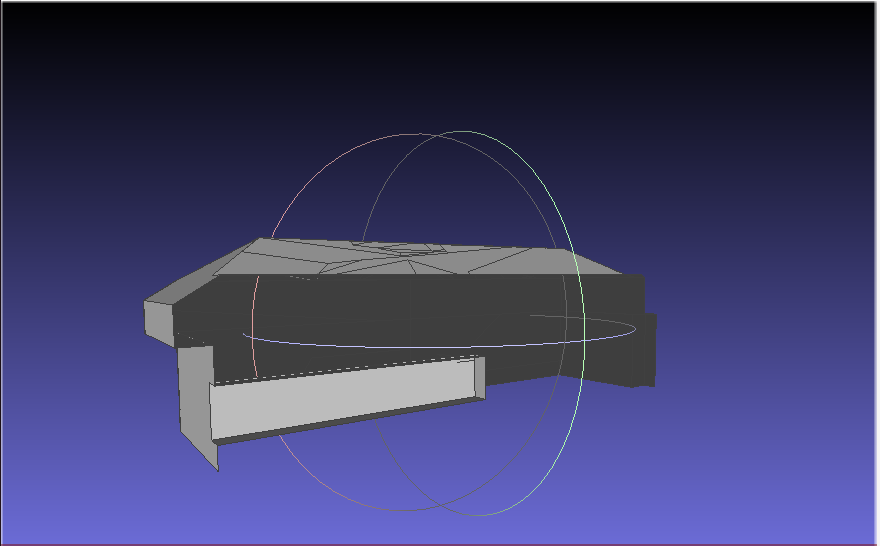
\includegraphics[width=\textwidth]{../images/screen_kinetic/back_dist001_pmin250.png}
        \caption{dist001\_pmin250}
        \label{fig:dist1_pmin300}
      \end{minipage}
  \end{figure}


  When considering the 'dist' parameter, if it is set too high, we risk losing significant structural details. 
  In the opposite, if the distance is too small, surfaces may be divided into too many planes, potentially resulting in an incomplete coverage of the entire mesh, 
  as observed at the rear of the building with a 'dist' of 0.001.

  One of the challenges in studying this algorithm is determining the appropriate 'qmin' and 'dist' to achieve the desired number of space partitions.
  Setting it too high may enhance precision but extend execution time, and in some cases, incorrect values can lead to program crashes.

This algorithm could be a crucial tool in our project, particularly when dealing with massive meshes for large buildings,
hospitals, etc. When creating large meshes, issues can arise, and errors within the mesh can be detrimental during simulations,potentially leading to false results. 
This algorithm allows us to rectify such mesh problems.

One limitation of the algorithm is its input requirement, as it currently only works with scatter plots. Consequently, we are unable to utilize the IFC format, 
resulting in the loss of valuable information regarding the types of structures present. To address this limitation, 
we plan to implement a process involving the conversion of IFC to scatter plot with associated data, followed by conversion to formats such as .plt, .ply, .xyz,
which are supported by Kinetic CGAL, ultimately resulting in a mesh with associated data.


\news


\subsection{Roadmap}
We intend to work on this project in the coming months and will continuously update our progress as outlined in the following roadmap.
\begin{figure}[h]
    
    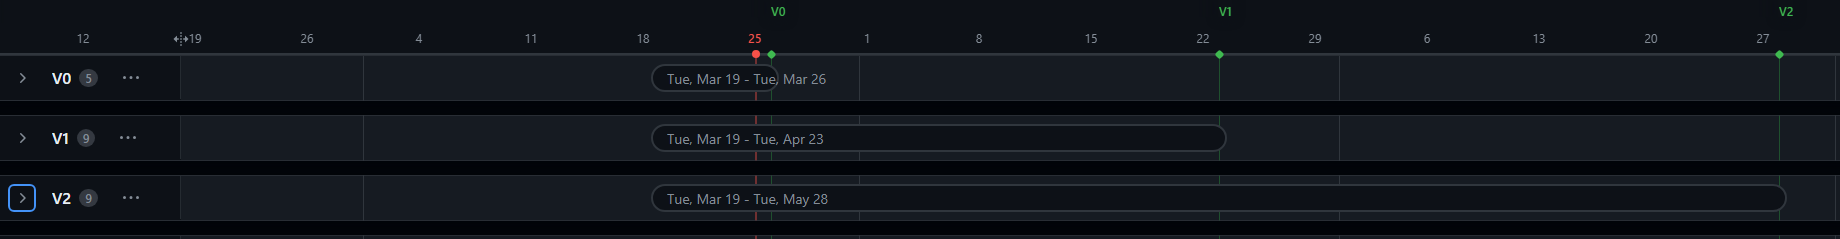
\includegraphics[scale =   0.3 ]{../images/roadmap.png}
    
\end{figure}
    
\nocite{*}
\bibliographystyle{plain}
\bibliography{../../bibliography/v0/report_bib}
\end{document}